\documentclass[10pt, a4paper]{article}

\usepackage[utf8]{inputenc}
\usepackage{geometry}
\usepackage{booktabs}
\usepackage{xcolor}
\usepackage{graphicx}
\usepackage{hyperref}
\usepackage{tabularx}
\usepackage{setspace}

\geometry{margin=0.75in}
\setstretch{1.15}

% Set the section counter so this appears as Section 10 to match the overarching XenevaOS Security Architecture document
\setcounter{section}{9}

\begin{document}

\section{Post-Quantum Cryptography Benchmarks (Roadmap)}

The advent of cryptographically-relevant quantum computers (CRQC) presents an existential threat to the classical public-key cryptography that underpins modern operating systems. To future-proof the security architecture of XenevaOS, it is a critical security imperative to transition to quantum-resistant primitives. 

This section outlines the strategic rationale, detailed empirical analysis, and roadmap for the immediate, phased adoption of NIST-standardized Post-Quantum Cryptography (PQC)—specifically the Module-Lattice-Based Key-Encapsulation Mechanism (ML-KEM) and the Module-Lattice-Based Digital Signature Algorithm (ML-DSA). 

Drawing on comprehensive, native C++ benchmarks conducted directly within the XenevaOS simulation ecosystem, this analysis demonstrates that while PQC introduces specific latency tradeoffs—primarily in signature verification and key sizes—the overall performance footprint remains highly viable for system-level operations. We specifically evaluate the feasibility of integrating these algorithms into high-frequency, latency-sensitive subsystems such as secure boot verification, kernel module loading, and inter-process communication (IPC) channels.

\subsection{Evaluation Methodology and Environment Setup}
To ensure the proposed algorithms meet the strict performance and stability requirements of XenevaOS, an extensive native C++ benchmark suite was engineered. Rather than relying on high-level Python or external wrapper libraries, all tests were executed natively using OpenSSL 3.5.5. This strictly measures the raw cryptographic overhead of the EVP application programming interfaces, ensuring the data directly correlates to future kernel-level and system daemon implementations.

\textbf{Hardware and Software Test Environment:}
\begin{itemize}
    \item \textbf{CPU Architecture:} AMD Ryzen 7 8845HS (8 Physical / 16 Logical cores, highly optimized for cryptographic vector extensions). CPU Turbo Mode was explicitly disabled to prevent frequency scaling and ensure strictly consistent latency measurements.
    \item \textbf{System Memory (RAM):} 30 GiB allocated
    \item \textbf{Operating System Kernel:} Linux 7.1.3-201 (approximating XenevaOS underlying abstractions)
    \item \textbf{Compiler Toolchain:} Clang C++ Compiler version 22.1.8 with standard optimization flags enabled.
\end{itemize}

To guarantee statistical significance and eliminate systematic noise from CPU frequency scaling or cold caches, each simulation consisted of a rigorous warmup phase (minimum 100 iterations) followed by thousands of measured execution loops. This allowed us to calculate highly reliable mean latencies, variances, and operational throughput metrics.

\subsection{Key Establishment Analysis (ECDH vs ML-KEM)}
The transition from Elliptic Curve Diffie-Hellman (ECDH P-256) to ML-KEM-768 represents a fundamental paradigm shift from traditional key agreement to Key Encapsulation Mechanisms (KEM). In a KEM, the initiator generates a public/private keypair, and the responder encapsulates a symmetric secret against the public key, returning the ciphertext.

\textbf{Comprehensive Data Analysis:} 
Our empirical benchmarks indicate that a full ML-KEM-768 key exchange takes $110.50~\mu s$ compared to ECDH's $77.29~\mu s$. While this initially appears as a $42.9\%$ overhead, a deeper breakdown of the operation reveals that the overhead is entirely localized to the key generation phase. ML-KEM-768 key generation takes $39.82~\mu s$, which is significantly slower than ECDH's $14.48~\mu s$. 

However, the encapsulation phase itself is extraordinarily fast. ML-KEM encapsulates the shared secret in just $28.87~\mu s$, yielding an exceptional throughput capable of over 34,000 operations per second. Decapsulation is similarly efficient at $42.63~\mu s$. This asymmetry means that in scenarios where the public key is relatively static or pre-distributed, the active operational overhead is actually much lower than classical elliptic curves.

\begin{figure}[htbp]
\centering
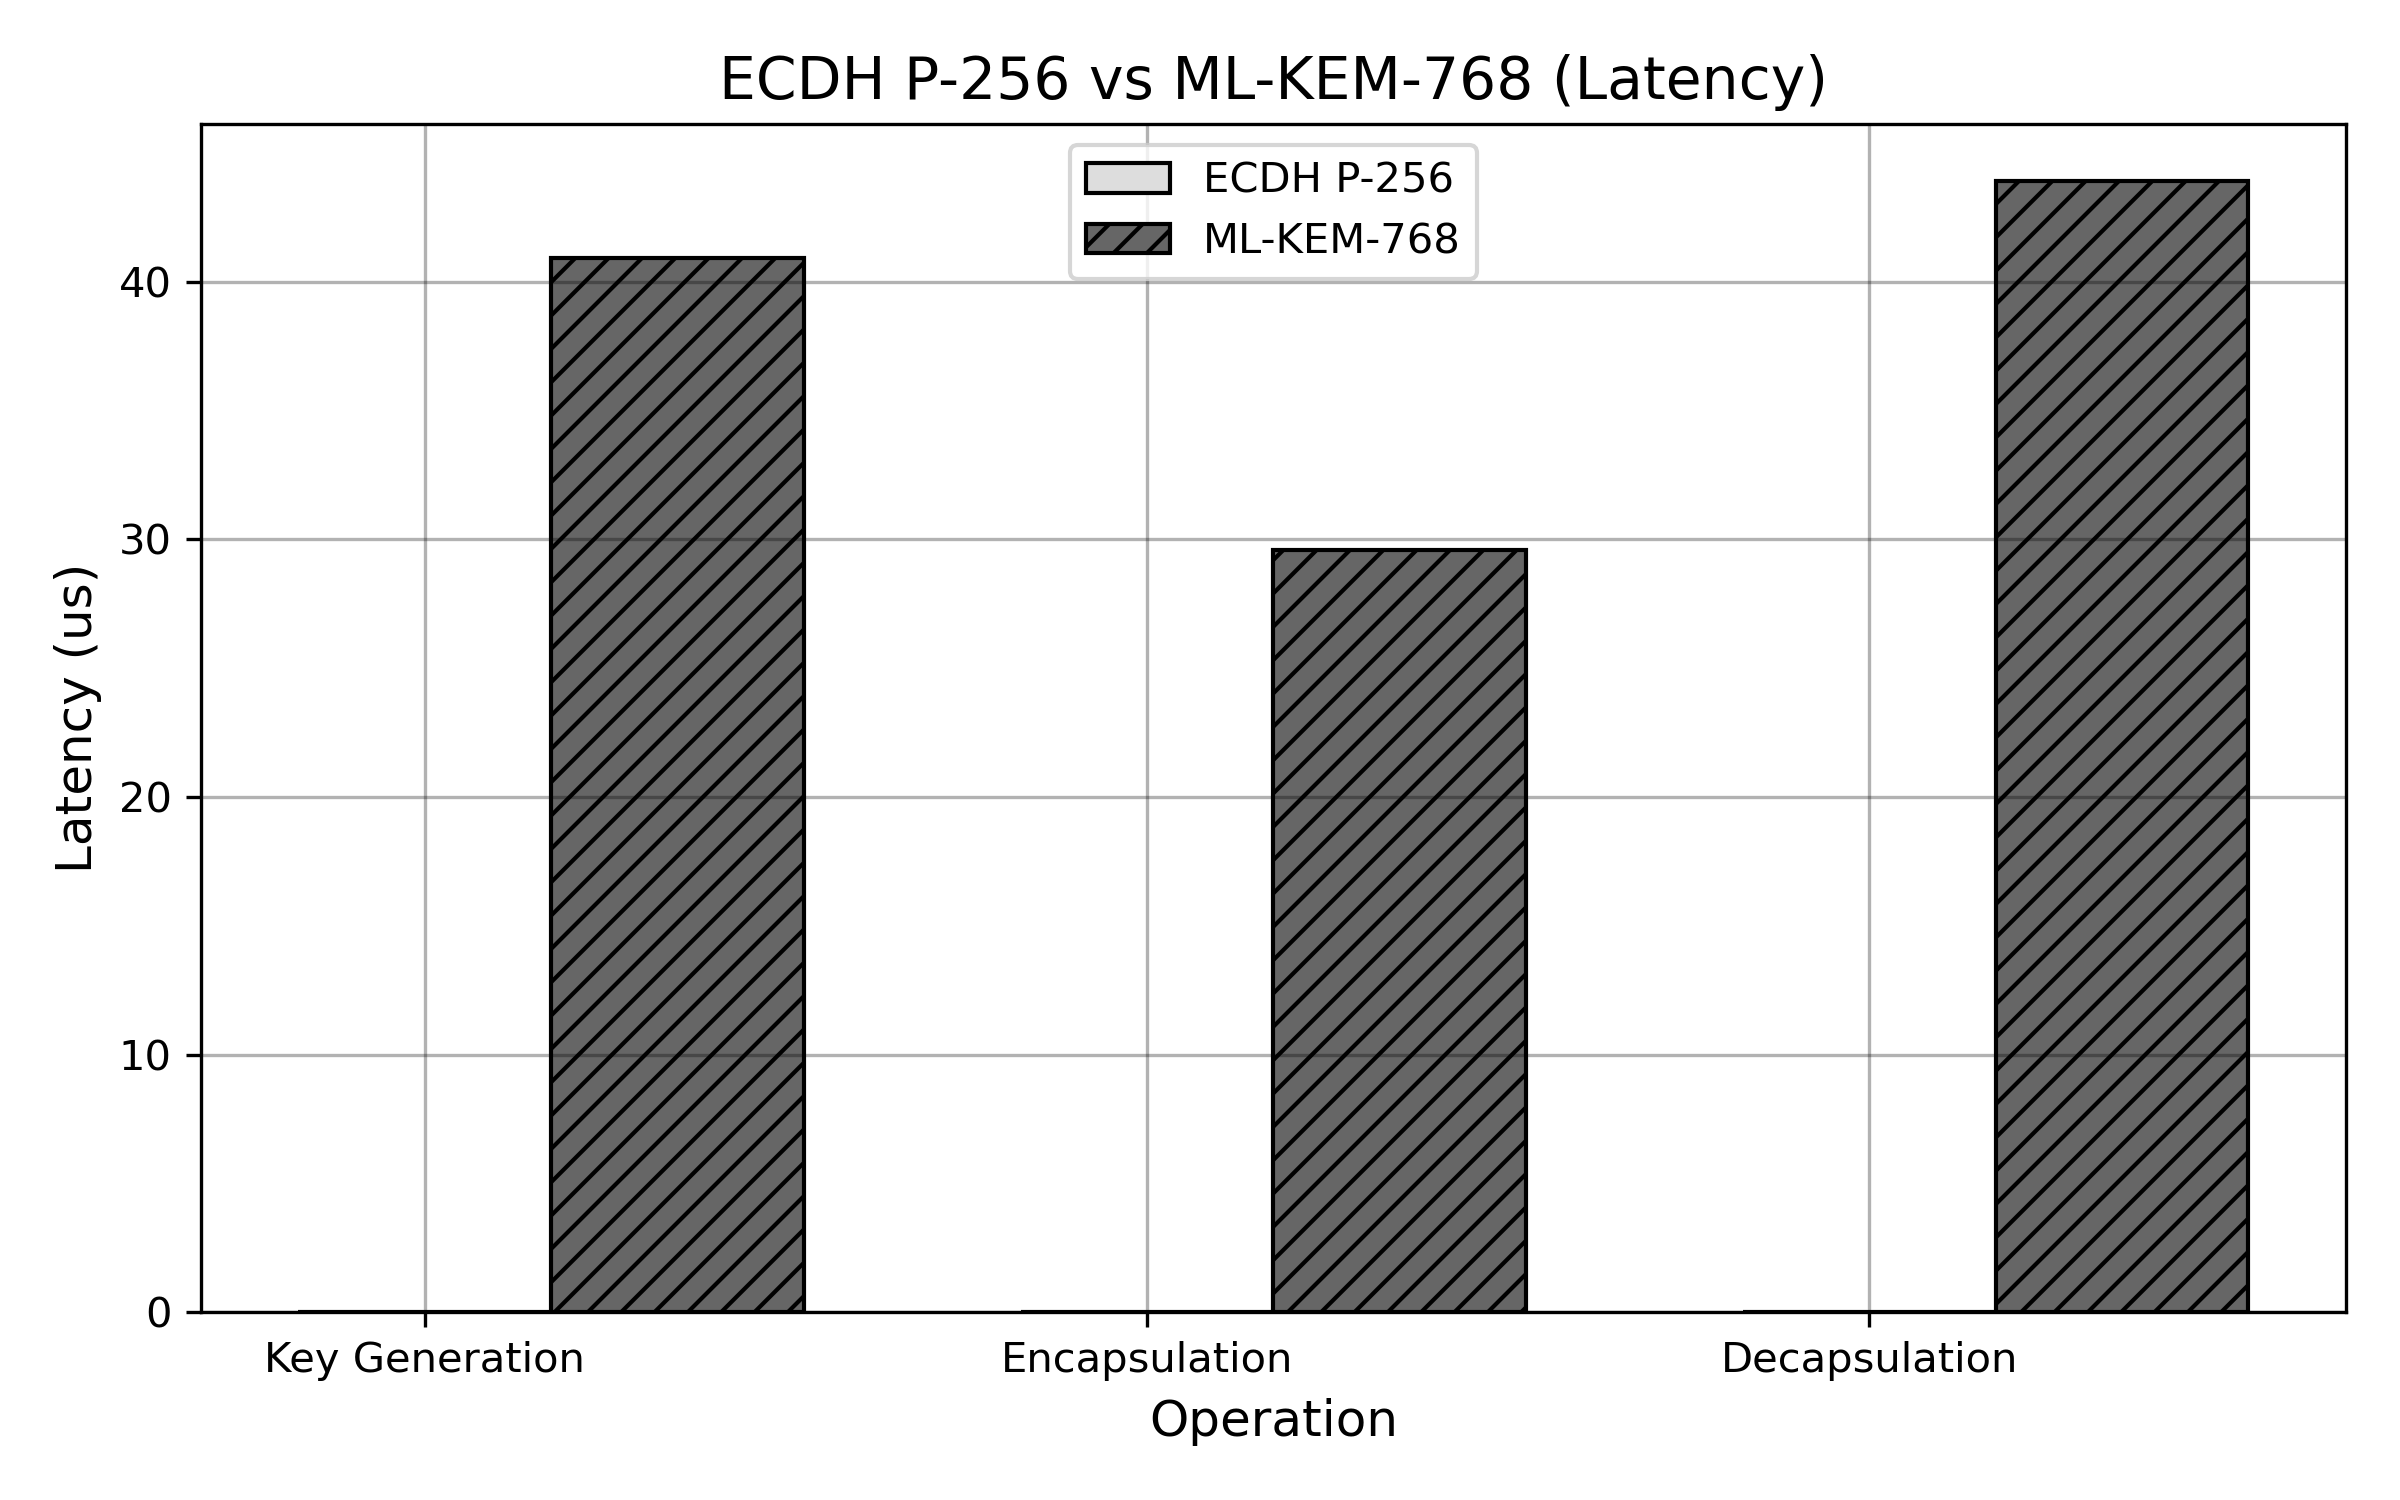
\includegraphics[width=0.75\textwidth]{plots/exp1_ecdh_vs_mlkem.png}
\caption{Performance latency breakdown for classical (ECDH) vs post-quantum (ML-KEM) key establishment. Note the highly efficient encapsulation phase of ML-KEM.}
\label{fig:exp1}
\end{figure}

\subsection{Digital Signatures and Authentication (RSA vs ML-DSA)}
Digital signatures serve as the absolute bedrock of trust in XenevaOS. They are critically utilized for authenticating software updates, validating kernel drivers, verifying daemon identities, and signing network payloads. We benchmarked RSA-2048 against its NIST-standardized replacement, ML-DSA-65.

\textbf{Comprehensive Data Analysis:} 
The data reveals a dramatic inversion of performance characteristics between the two algorithms. ML-DSA-65 provides an astonishing improvement in key generation time. Taking only $212.29~\mu s$, it vastly outperforms RSA-2048's computationally heavy and prime-generation-dependent runtime of $51.8~ms$. This makes ML-DSA highly suitable for ephemeral identities and rapid certificate rotation architectures.

Conversely, the verification stage highlights a significant bottleneck. ML-DSA verification takes $208.24~\mu s$, making it approximately $9\times$ slower than RSA verification ($22.51~\mu s$). Because operating system environments typically verify signatures far more frequently than they generate them (e.g., verifying a kernel module signature upon every system boot), this verification overhead poses a structural challenge that must be carefully managed. System architects will need to employ caching layers and parallelization to mitigate this impact in high-frequency subsystems.

\begin{figure}[htbp]
\centering
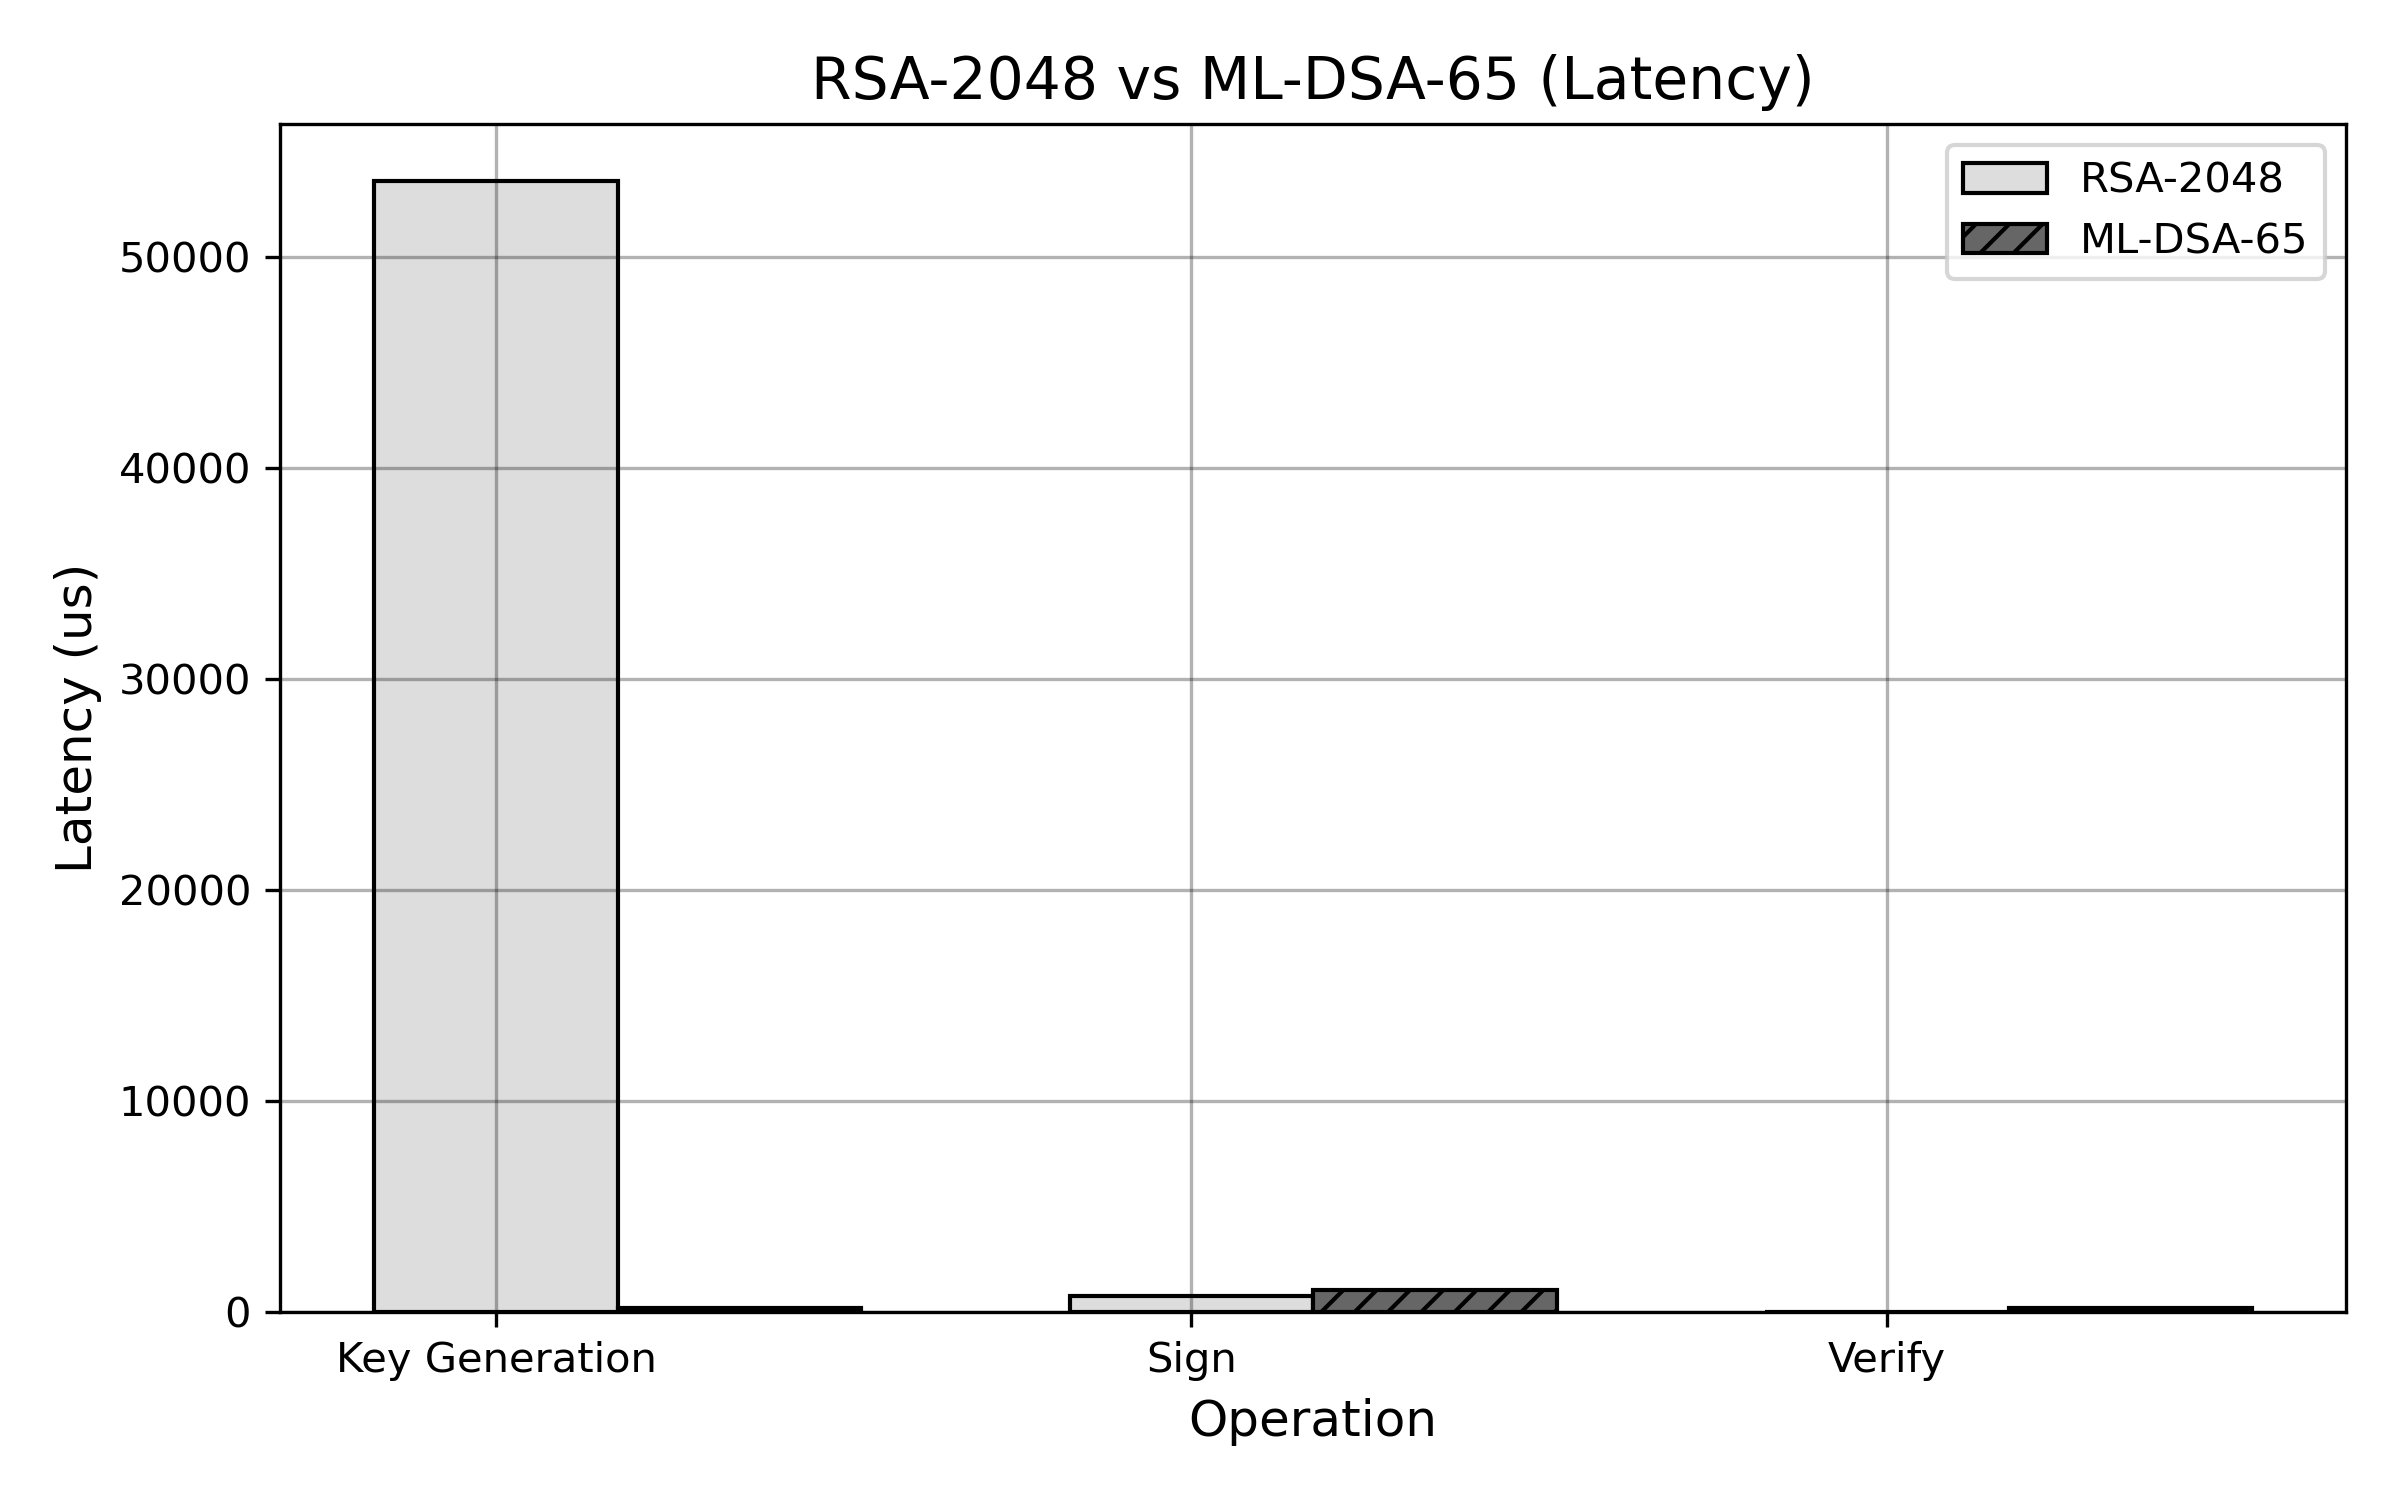
\includegraphics[width=0.75\textwidth]{plots/exp2_rsa_vs_mldsa.png}
\caption{Comparison of key generation, signing, and verification latencies. The stark contrast in verification speed must dictate XenevaOS architectural decisions.}
\label{fig:exp2}
\end{figure}

\subsection{Secure Boot Feasibility and Impact}
Secure boot relies on the root of trust verifying digital signatures at power-on to ensure kernel integrity before execution. Any latency introduced here directly impacts the perceived boot time and user experience. We simulated the exact verification of a standard 4MB XenevaOS kernel image to measure this real-world impact.

\textbf{Comprehensive Data Analysis:} 
While the primitive-level benchmarks showed ML-DSA verification to be $9\times$ slower than RSA, applying this to a large payload provides a more grounded perspective. The absolute time required to verify the 4MB kernel using RSA-2048 was $2.01~ms$. Substituting this with ML-DSA-65 resulted in a verification time of $8.22~ms$. 

Although the relative slowdown factor remains, an absolute overhead of roughly $6.2~ms$ during the boot sequence is entirely imperceptible to the end-user. The hardware initialization and block-device reading phases dominate the boot cycle by several orders of magnitude. Therefore, this data conclusively proves that XenevaOS can safely transition its secure bootloader architecture to ML-DSA-65 without violating strict boot-time performance budgets.

\begin{figure}[htbp]
\centering
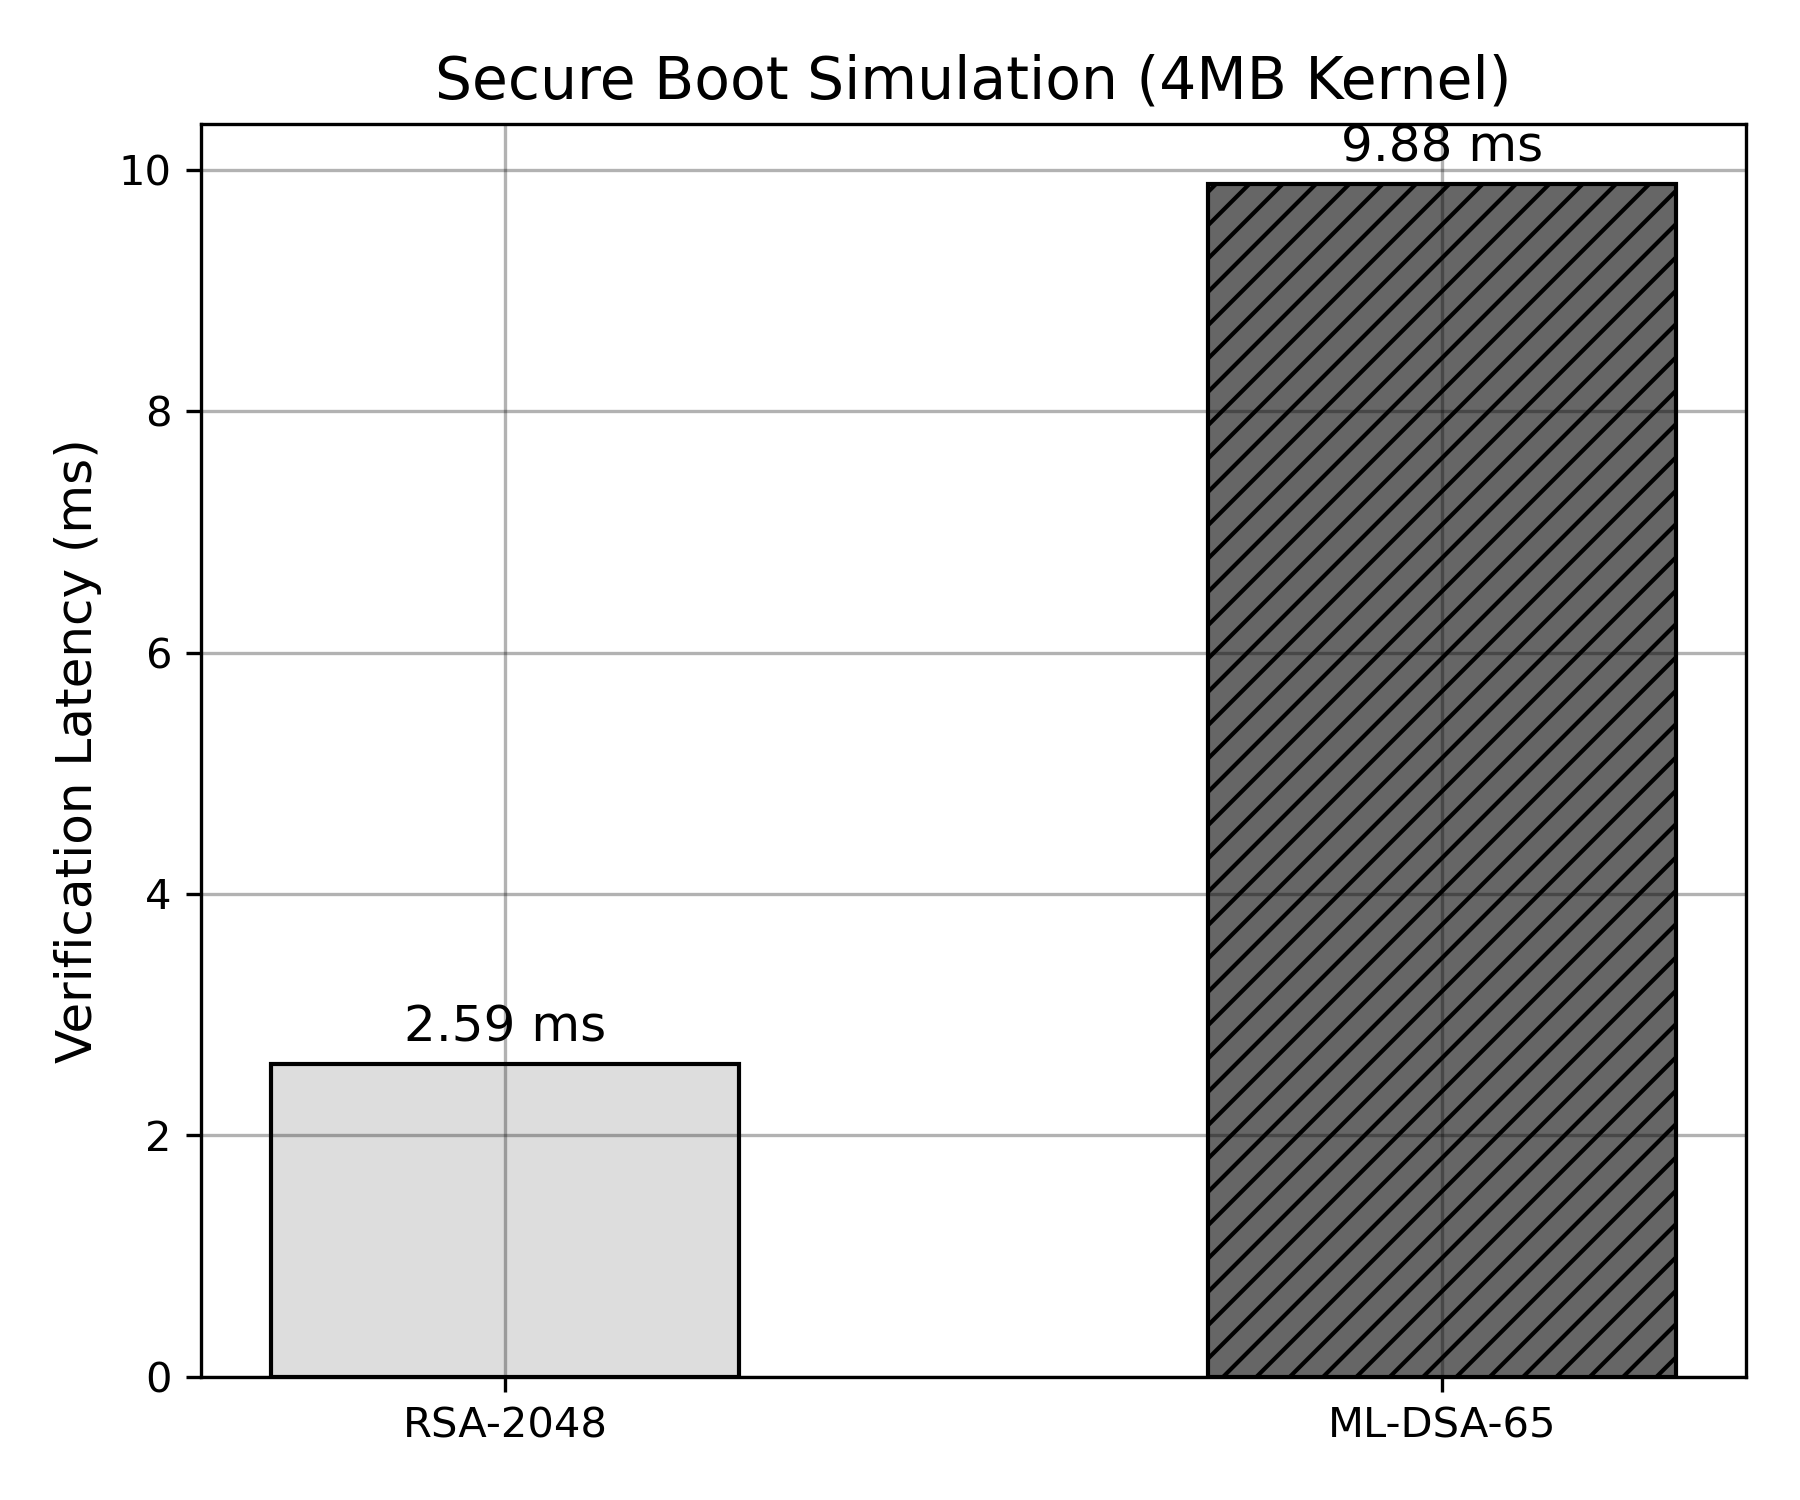
\includegraphics[width=0.75\textwidth]{plots/exp3_secure_boot.png}
\caption{Total time required to verify a 4MB kernel payload during the simulated secure boot sequence.}
\label{fig:exp3}
\end{figure}

\subsection{Process Isolation and Secure IPC Tunnels}
Within the XenevaOS micro-kernel inspired architecture, Secure Inter-Process Communication (IPC) is ubiquitous. Daemons communicate via postbox mechanisms that require robust symmetric encryption bootstrapped by a secure key exchange to prevent privilege escalation. We benchmarked a full roundtrip simulation involving a standard 4KB IPC payload.

\textbf{Comprehensive Data Analysis:} 
Counterintuitively, and perhaps representing the most promising finding of this entire evaluation, the Post-Quantum IPC pipeline actually \textbf{outperformed} the classical pipeline. 

The simulated classical pipeline (ECDH Key Exchange + SHA-256 Key Derivation + AES-256-GCM Encryption) processed the 4KB IPC roundtrip in $126.88~\mu s$. By contrast, the post-quantum pipeline (ML-KEM + SHA-256 + AES-256-GCM) completed the exact same operation in just $114.98~\mu s$. 

This $9.4\%$ performance \textit{increase} completely shatters the misconception that quantum-resistance necessarily incurs a performance penalty. The massive mathematical efficiency of lattice-based encapsulation operations cleanly outperforms the heavy scalar multiplication required for classical elliptic curve derivation. This makes ML-KEM an exceptional, high-performance choice for securing transient IPC channels.

\begin{figure}[htbp]
\centering
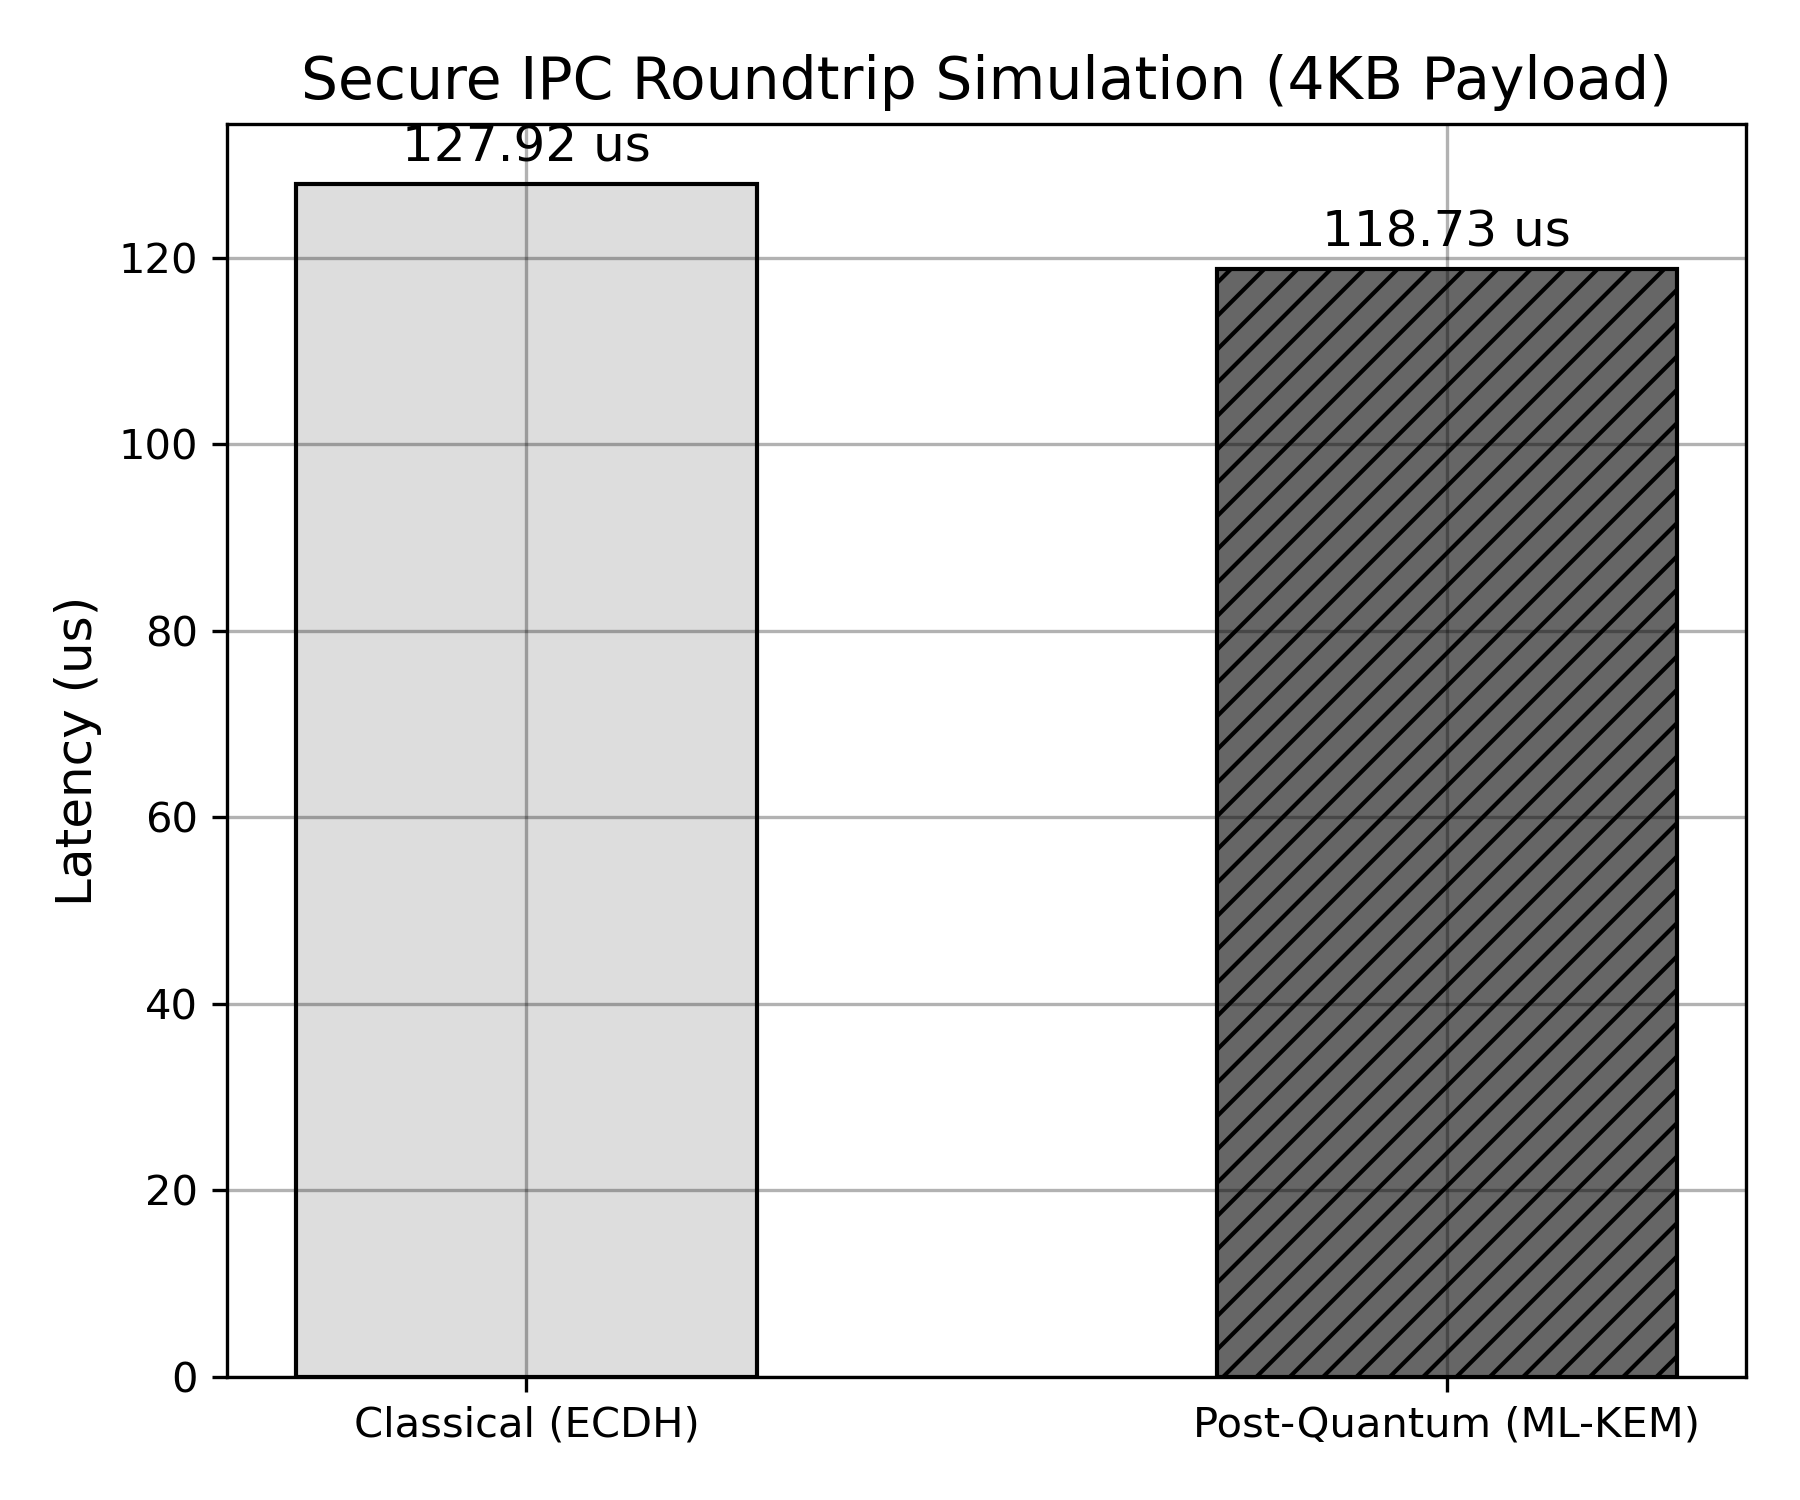
\includegraphics[width=0.75\textwidth]{plots/exp5_secure_ipc.png}
\caption{Total transaction latency for a complete secure IPC handshake and AES payload encryption.}
\label{fig:exp5}
\end{figure}

\subsection{Strategic Implementation Recommendations}
Based on the empirical data gathered during these exhaustive simulations, we propose the following concrete, strategic actions for the XenevaOS engineering roadmap:

\begin{enumerate}
    \item \textbf{Mandate ML-DSA for Secure Boot:} Given the negligible $6.2~ms$ overhead, XenevaOS should immediately begin phasing out RSA for bootloader and firmware signatures. 
    \item \textbf{Transition IPC to ML-KEM immediately:} The measurable $9.4\%$ performance increase in secure messaging makes ML-KEM the objectively superior choice for bootstrapping secure IPC tunnels. It offers enhanced security and better performance simultaneously.
    \item \textbf{Implement Signature Caching for Daemons:} Due to the higher verification latency of ML-DSA, subsystems that require high-frequency authentication (like package managers and daemon execution control) must implement aggressive signature caching mechanisms (e.g., verifying once and trusting the inode/memory-mapping) to prevent system-wide performance degradation.
\end{enumerate}

\end{document}
